\documentclass[border=4pt]{standalone}
\usepackage{tikz}
\usepackage{pgfplots}
\pgfplotsset{compat=1.18}
\usetikzlibrary{shapes.geometric,arrows.meta,positioning,calc,fit,decorations.pathreplacing,backgrounds}
\definecolor{boxblue}{RGB}{225,238,252}
\definecolor{boxgreen}{RGB}{225,247,231}
\definecolor{boxorange}{RGB}{253,236,216}
\definecolor{boxgray}{RGB}{237,237,237}
\definecolor{boxred}{RGB}{253,226,226}
\begin{document}
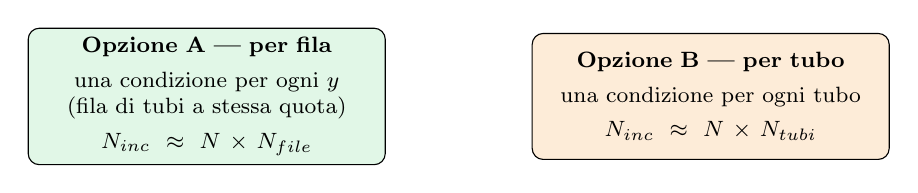
\begin{tikzpicture}[
  box/.style={draw, rectangle, rounded corners, minimum height=1.6cm, text width=4.3cm, align=center, font=\footnotesize},
]
\node[box, fill=boxgreen] (a) at (-3.2,0) {\textbf{Opzione A — per fila}\\[3pt] una condizione per ogni $y$ (fila di tubi a stessa quota)\\[3pt] $N_{inc} \approx N \times N_{file}$};
\node[box, fill=boxorange] (b) at (3.2,0) {\textbf{Opzione B — per tubo}\\[3pt] una condizione per ogni tubo\\[3pt] $N_{inc} \approx N \times N_{tubi}$};
\end{tikzpicture}
\end{document}
